To ensure that the cosmology extracted using the
halo mass function as measured on galaxy clusters
using weak lensing is accurate, it is important that
galaxy clusters at various redshifts have 
similar levels of shape measurement bias. The population of 
galaxies observed at different redshifts will vary in
S/N, ellipticity distribution, size and morphology;
all properties which can effect the accuracy of a lensing 
measurement. The bias of galaxy sources with S/N $>$ 
20 as a function of redshift is shown in Figure \ref{fig:red}.
The results of bias of the lensing pipelines was quantified 
by fitting for M and C . 

\begin{figure}
 \centering  % this centres figure in column
  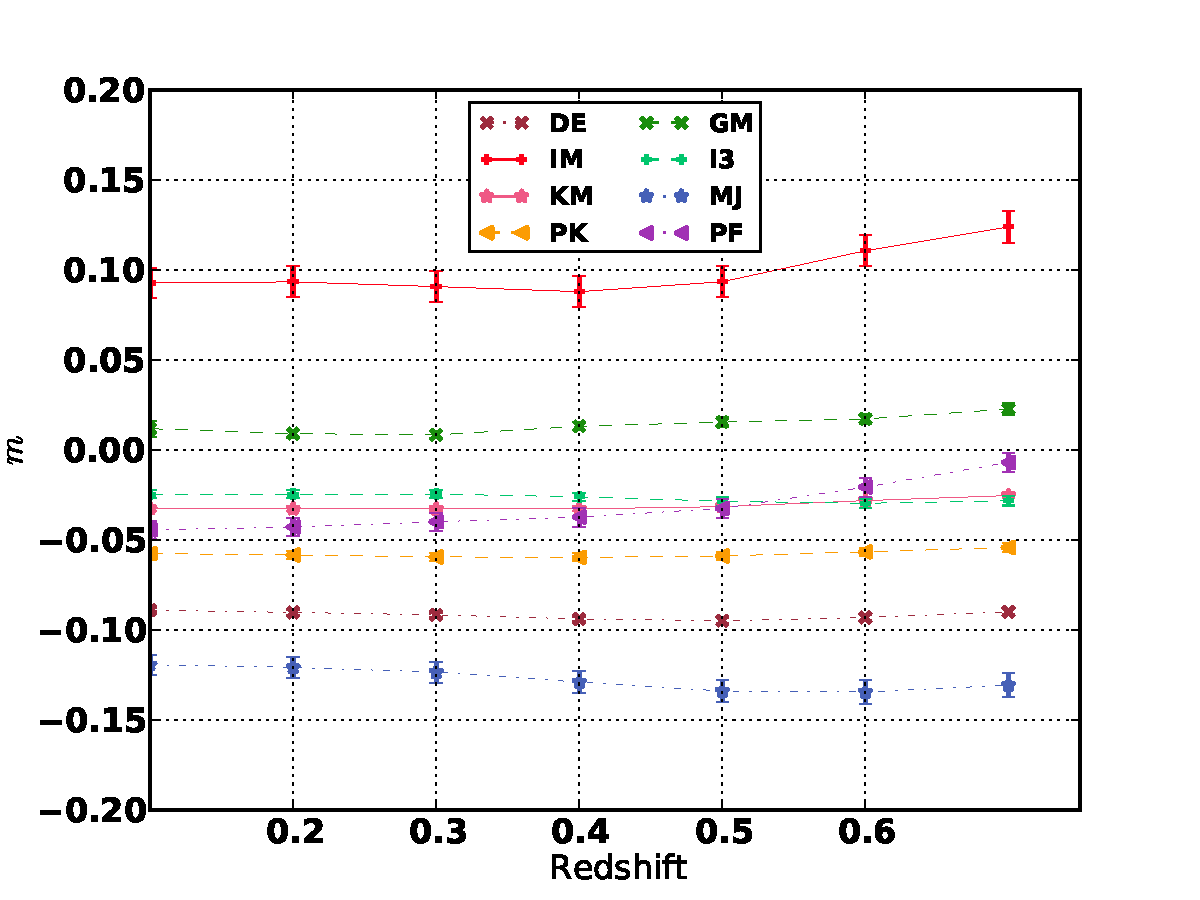
\includegraphics[width=0.45\textwidth]{fig/Mvalred_mfix.pdf} 
  \caption{Multiplicative shape measurement
  bias (M) of pipelines as a function of redshift.}
\label{fig:red}
\end{figure}
We find that MJ, DE, PK, I3 and KM
show a consistent level of shape measurement bias as a function of 
redshift. Our results are consistent with an analysis 
that studied the shape measurement bias as a function of redshift for I3 
\citep{K_2} on simulated COSMOS galaxies
and determined that it did not not vary significantly as a function
of redshift. 

